\section{Umsetzung}\label{sec:umsetzung}

    \subsection{Resultate}

        Das Praxisrufsystem wurde wie im Kapitel 5 - Konzept beschrieben umgesetzt.
Es wurden die drei Komponenten Mobile Client, Cloud Service und Admin UI implementiert.
Über den angebundenen Messaging Service Firebase Messaging ist es möglich, Benachrichtigungen zwischen Mobile Clients zu versenden.
Cloud Service und Admin UI ermöglichen es dabei die Benachrichtigungen die Versendet werden können und welcher Client welche Benachrichtungen erhalten soll zu konfigurieren.
Weiter wurde mit Amazon Web Services (AWS) eine CI/CD Umgebung aufgebaut, die es erlaubt Cloud Service und das Admin UI zu betreiben und testen.
Diese Umgebung wird dem Kunden als Template dienen, wie er das Praxisrufsystem in der Praxis betreiben kann\footnote{Siehe Anhang Betriebshandbuch}.

Im Rahmen des Projektes wurden damit die Milestones M01 bis M06\footnote{Siehe Kapitel 2.2} erreicht.
Umgesetzt wurden die Milestones mit den folgenden User Stories inklusive aller dazu definierten Features und Szenarien\footnote{Siehe Kapitel 3}:

\begin{itemize}
    \item U01 - Benachrichtigung versenden
    \item U02 - Benachrichtigungen empfangen
    \item U03 - Nur relevante Benachrichtigungen empfangen
    \item U04 - Auf Benachrichtigungen aufmerksam machen
    \item U05 - Verpasste Benachrichtigungen anzeigen
    \item U06 - Fehler beim Versenden von Benachrichtigungen anzeigen
    \item U07 - Konfiguration auf Mobile Client auswählen
    \item U12 - Mehrere Mobile Clients konfigurieren
    \item U13 - Individuelle Konfiguration pro Mobile Client
    \item U14 - Zentrale Konfigurationsverwaltung
    \item T01 - Mobile Client unterstützt IPads
    \item T02 - Mobile Client unterstützt Android Tablets
    \item T03 - Geteilte Code Basis für Android and IOS
    \item T04 - Betrieb mit AWS
\end{itemize}

Die Milestones M06 bis M10 konnten im Rahmen dieses Projektes nicht umgesetzt werden.
Damit sind folgende User Stories ausserhalb des Projektrahmens gefallen:

\begin{itemize}
    \item U08 - Physicher Knopf am Behandlungsstuhl
    \item U09 - Text To Speech für Benachrichtigungen
    \item U10 - Direkte Unterhaltungen zwischen Mobile Clients
    \item U11 - Gruppenunterhaltungen zwischen Mobile Clients
    \item U15 - Konfiguration von direkten Anrufen
    \item U16 - Konfiguration von Gruppenanrufen
\end{itemize}

        \subsubsection{Mobile Client}\label{subsec:mobile-client-realisation}

Dieses Kapitel zeigt die umgesetzten Ansichten des Mobile Clients.
Weitere Informationen zur Bedienung des Mobile Clients sind dem Benutzerhandbuch zu entnehmen\footnote{Siehe Anhang C}.

\subsubsection*{Anmeldung und Konfiguration}

Wird die Mobile Client Applikation zu ersten Mal geöffnet, muss die korrekte Konfiguration geladen werden.
So können Buttons für die benötigten Benachrichtigungen angezeigt und relevante Benachrichtigungen empfangen werden.
In einem ersten Schritt wird dem Benutzer deshalb eine einfache Login-Maske angezeigt.
Darin kann sich der Benutzer mit Benutzername und Passwort anmelden.
War die Anmeldung erfolgreich, werden alle Konfigurationen geladen, die dem Benutzer zur Verfügung stehen.
Die verfügbaren Konfigurationen werden dem Benutzer in einer Liste angezeigt und er wird aufgefordert, die gewünschte Konfiguration auszuwählen.
Nachdem die Auswahl erfolgt ist, wird der Benutzer zur Startseite weitergeleitet.

\begin{figure}[h]
    \centering
    \begin{minipage}[b]{0.4\textwidth}
        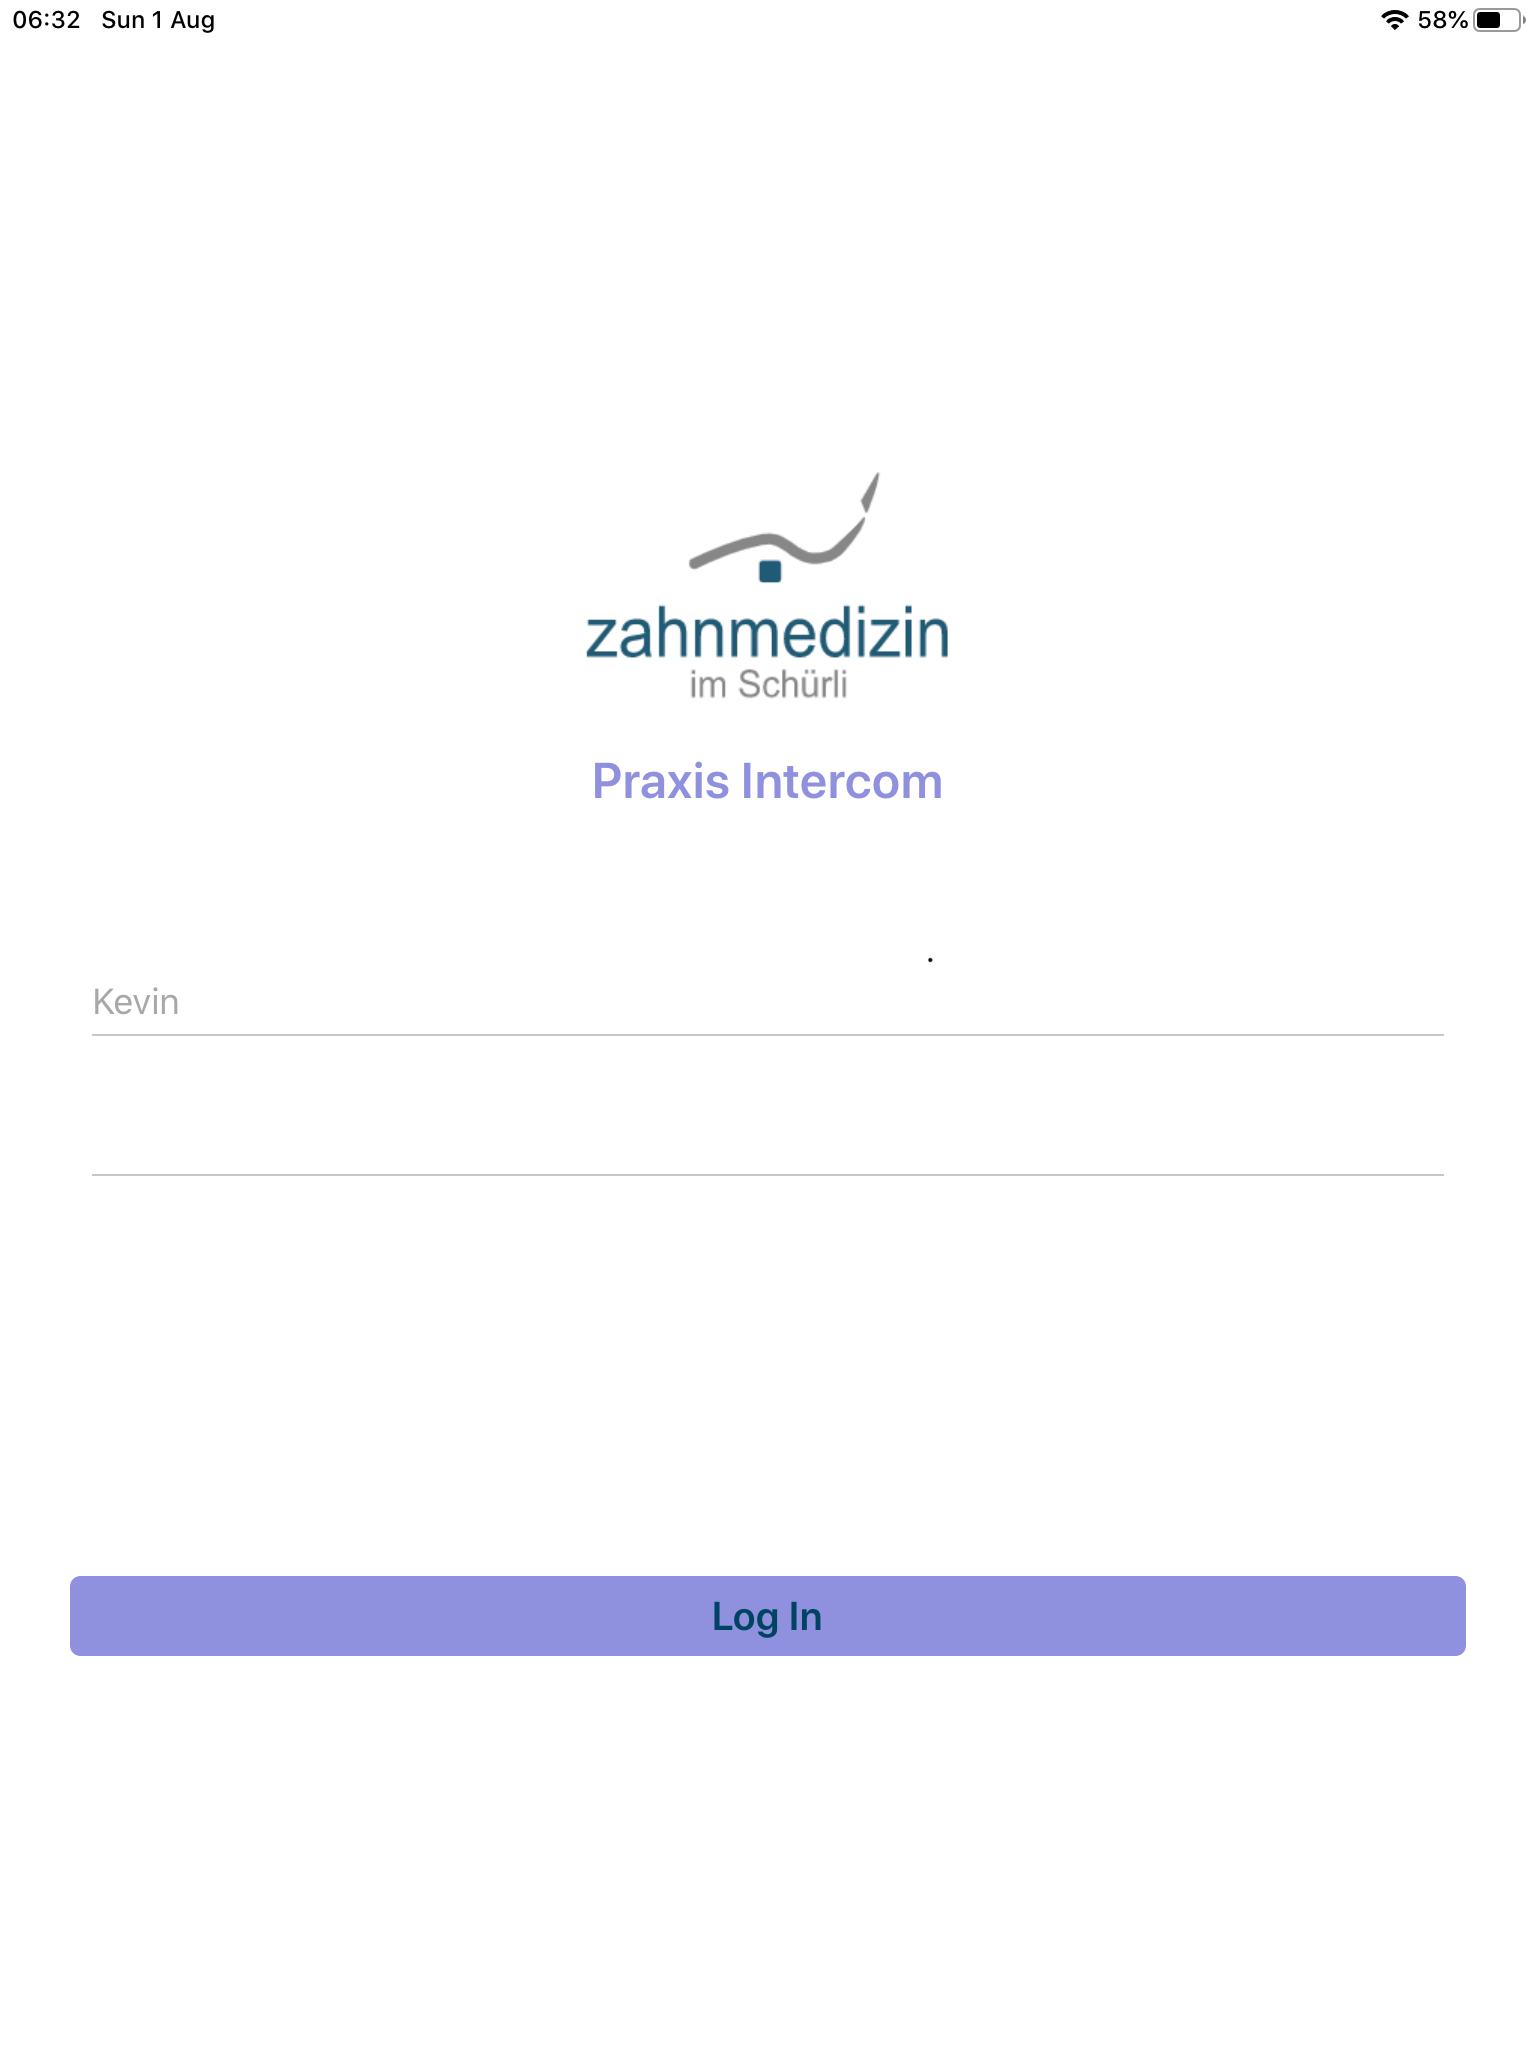
\includegraphics[width=\textwidth]{graphics/screenshots/mobileclient/screenshots-login}
        \caption{Login}
    \end{minipage}
    \hfill
    \begin{minipage}[b]{0.4\textwidth}
        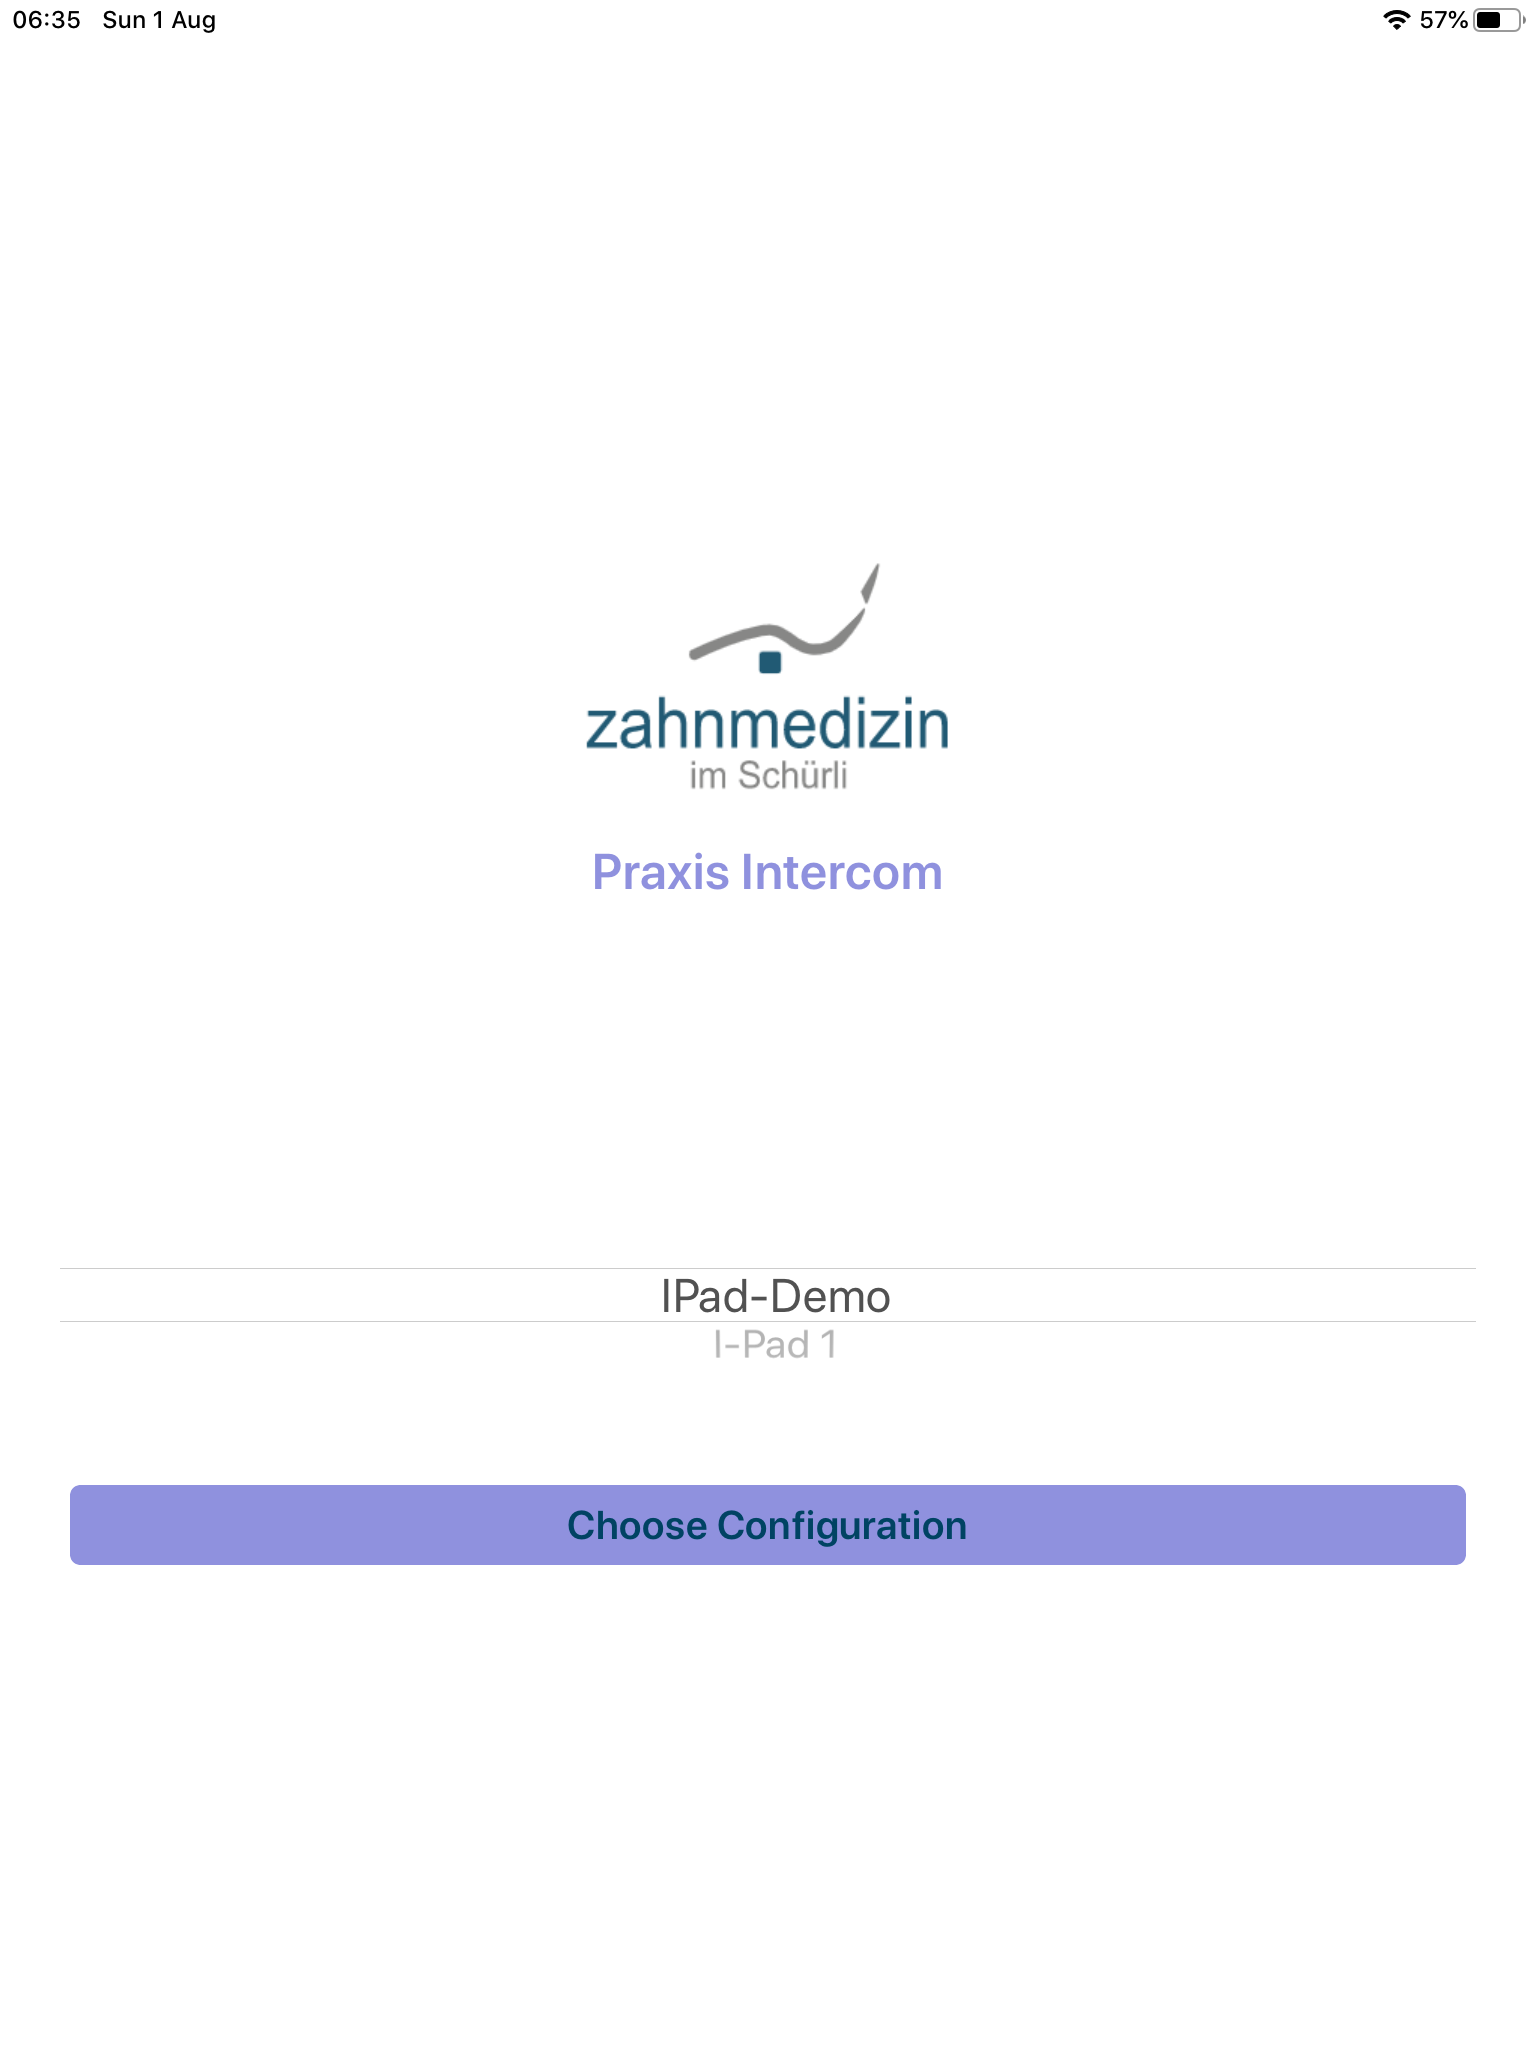
\includegraphics[width=\textwidth]{graphics/screenshots/mobileclient/screenshot-select-config}
        \caption{Konfiguration}
    \end{minipage}
    \label{fig:MobileClient-Screens1}
\end{figure}

\clearpage

\subsubsection*{Benachrichtigungen versenden}

Im Tab Home der Startseite werden Buttons angezeigt, um Benachrichtigungen zu versenden.
Die Buttons werden dynamisch aus der geladenen Konfiguration generiert.
Dabei gibt die Konfiguration den Text vor, der auf dem Button angezeigt wird.
Der Inhalt der Benachrichtigung, die der Button auslöst, ist in der Konfiguration im Cloud Service hinterlegt.

Tippt der Benutzer auf einen der Buttons, wird die entsprechende Benachrichtigung versendet.
Die Vermittlung, an die relevanten Empfänger übernimmt dabei der Cloud Service.
Dieser entscheidet anhand der vorhandenen Konfiguration, welchen Clients die Benachrichtigung zugestellt wird.
Schlägt das Versenden der Benachrichtigung an mindestens einen Empfänger fehl, wird dies dem Benutzer angezeigt.
Der Benutzer hat dann die Möglichkeit, das Versenden an diese Empfänger wiederholen.

\begin{figure}[h]
    \centering
    \begin{minipage}[b]{0.4\textwidth}
        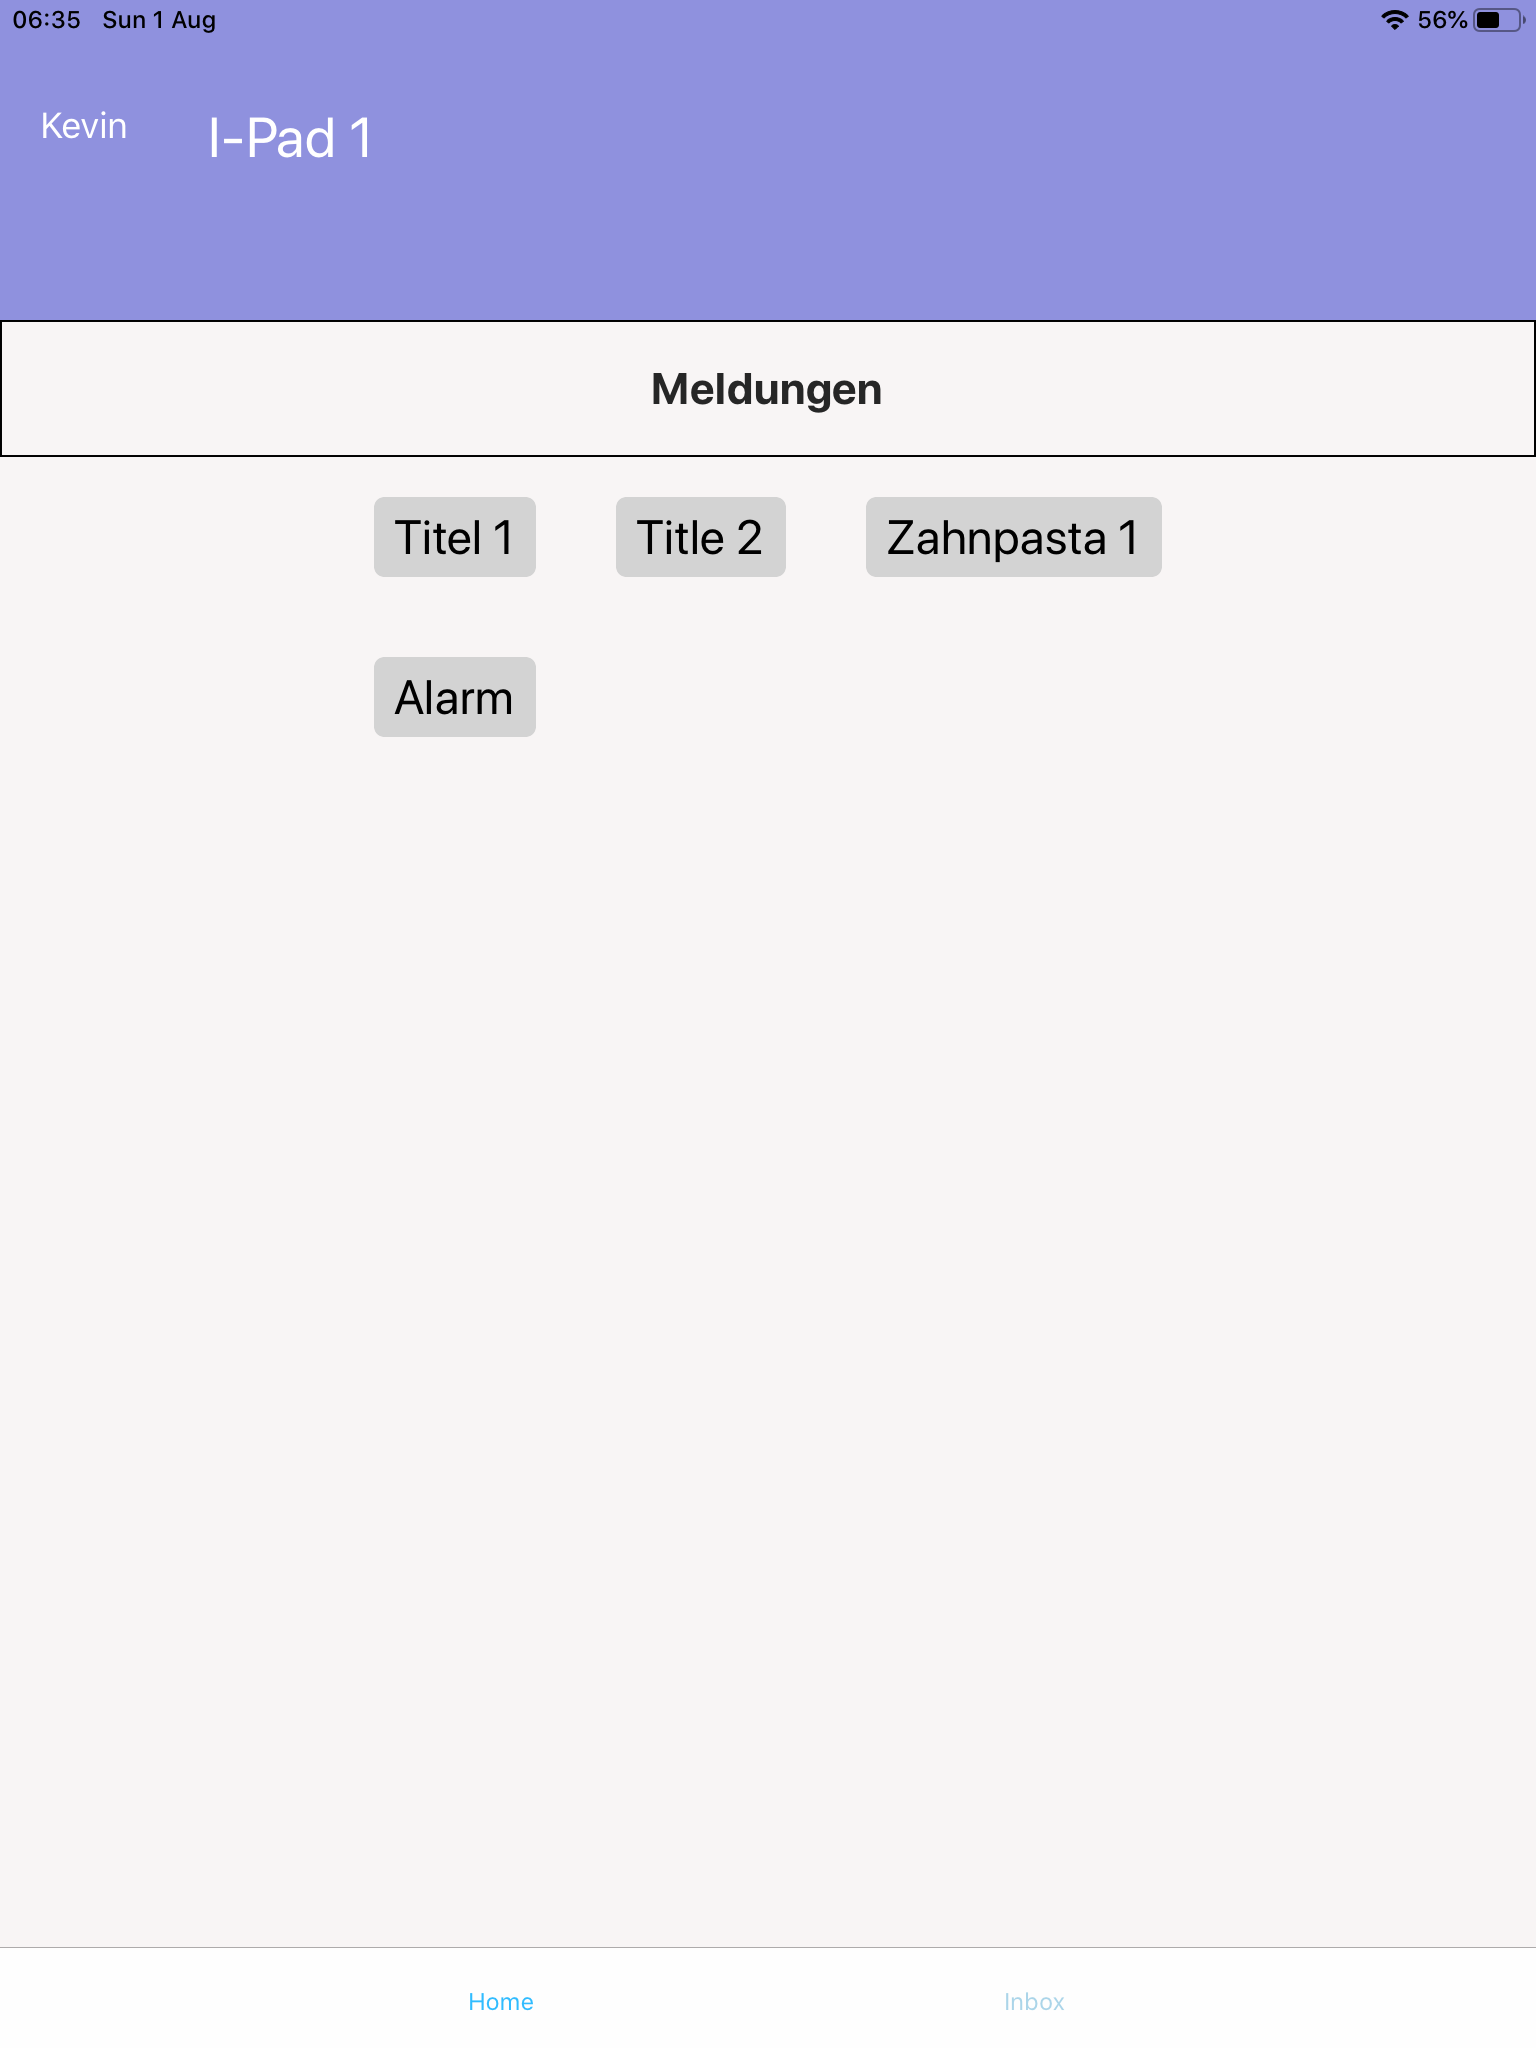
\includegraphics[width=\textwidth]{graphics/screenshots/mobileclient/screenshot-homescreen}
        \caption{Home}
    \end{minipage}
    \hfill
    \begin{minipage}[b]{0.4\textwidth}
        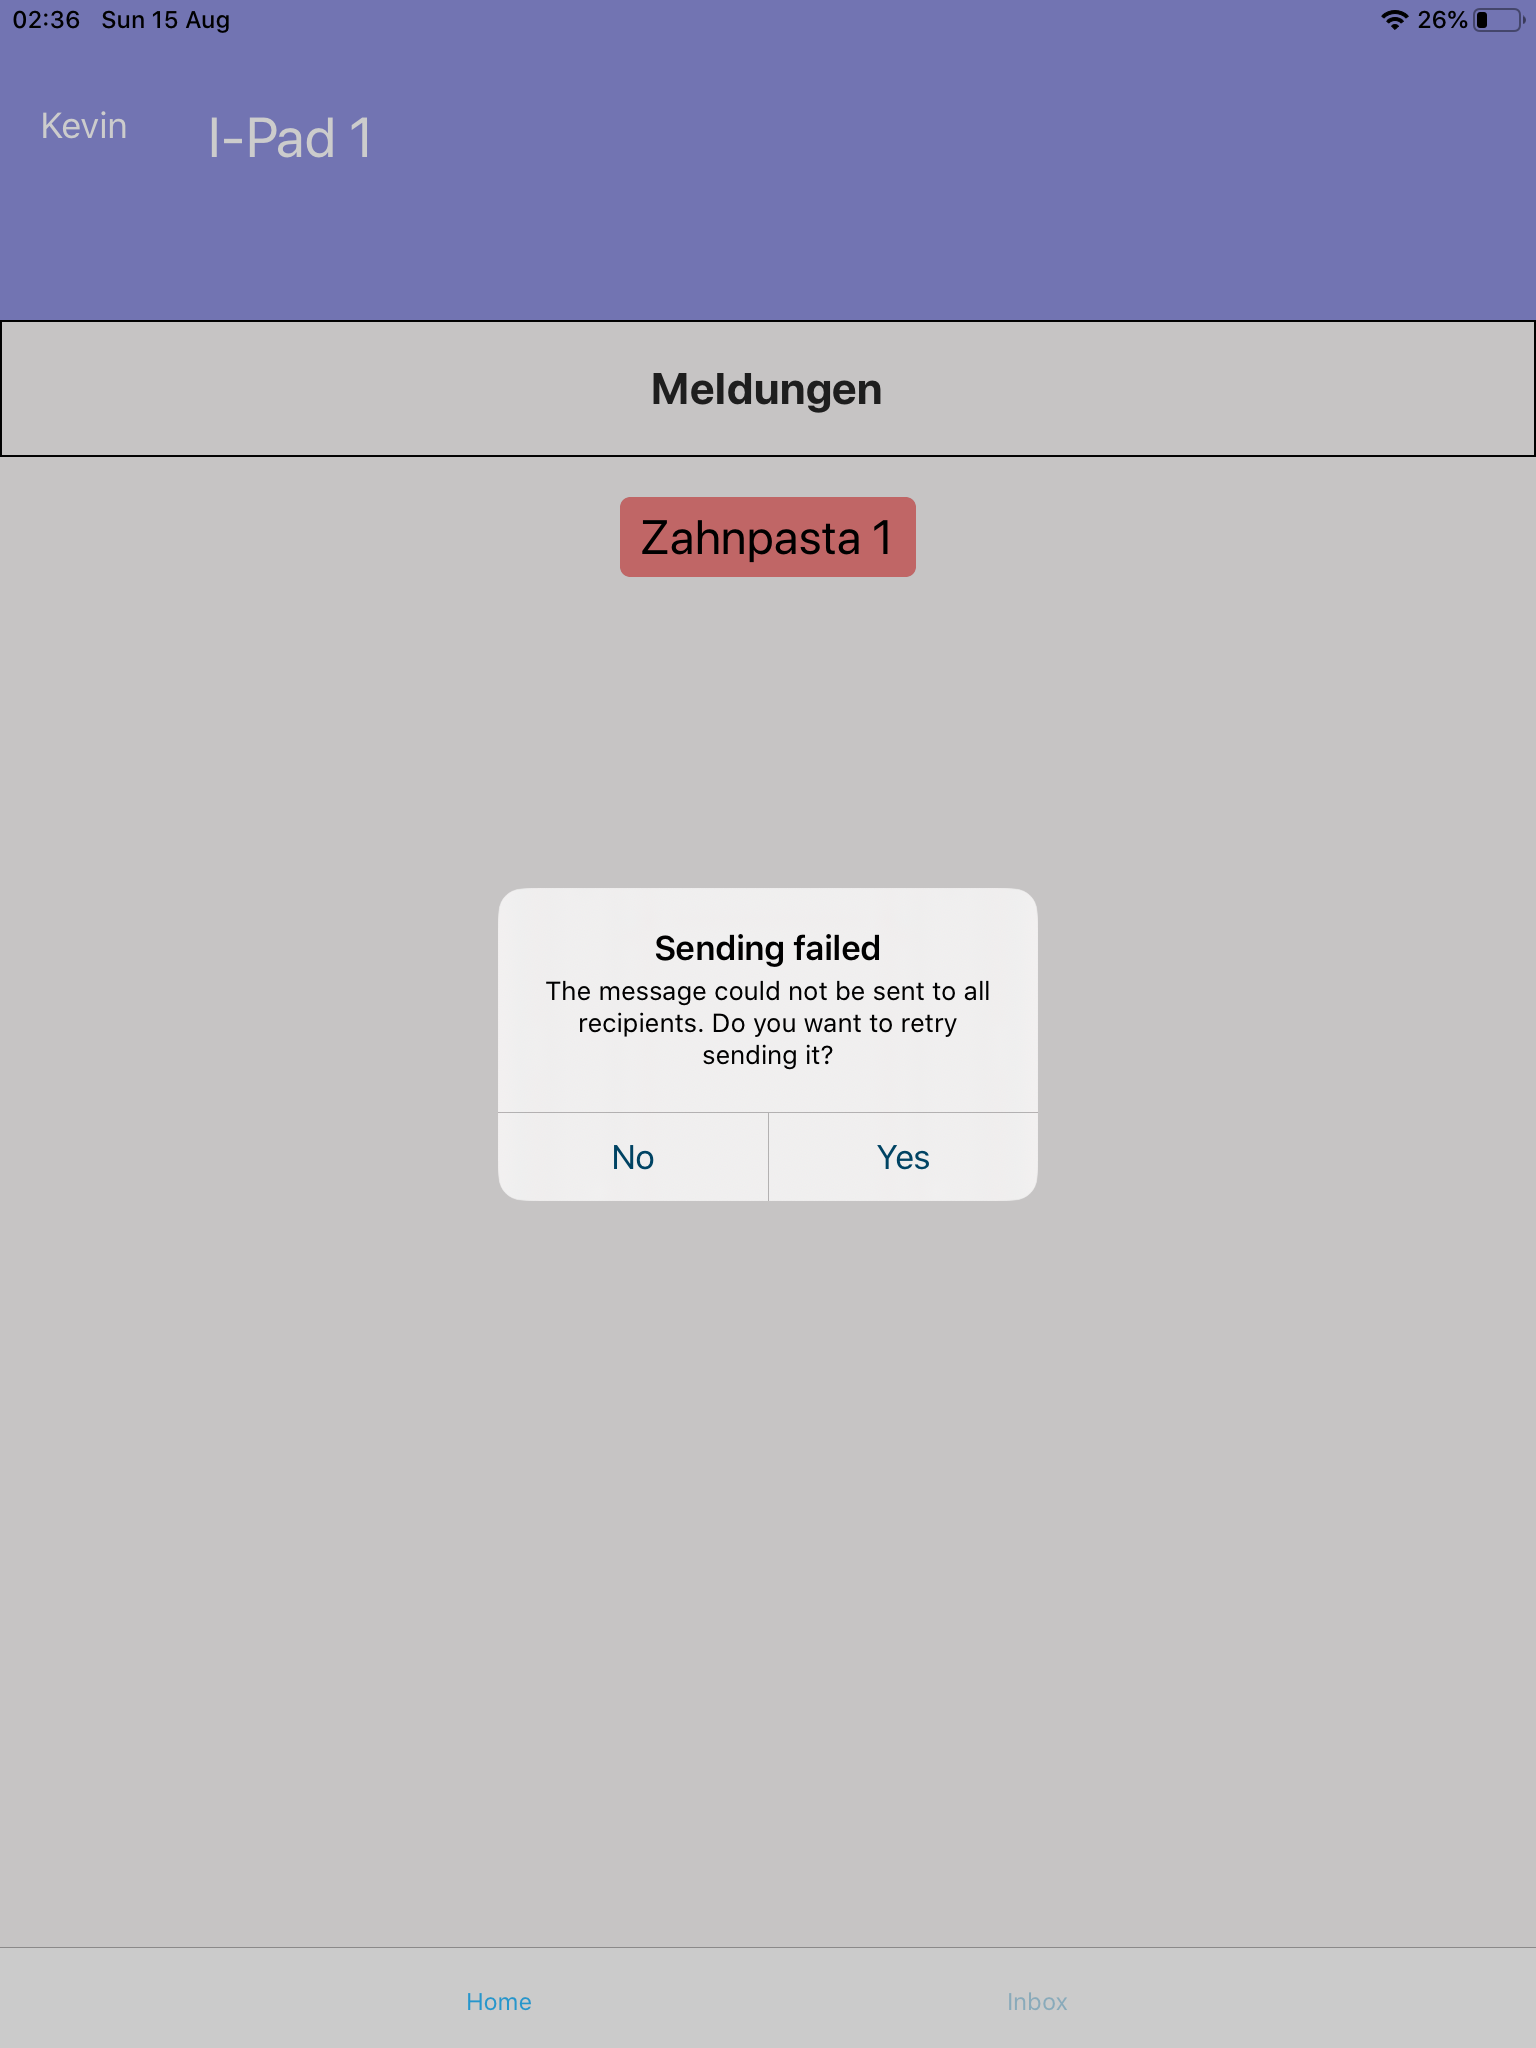
\includegraphics[width=\textwidth]{graphics/screenshots/mobileclient/screenshot-retry}
        \caption{Retry}
    \end{minipage}
    \label{fig:MobileClient-Screens2}
\end{figure}

\clearpage

\subsubsection*{Benachrichtigungen empfangen}

Wurde eine Benachrichtigung empfangen, ertönt ein Audio Signal und die Benachrichtigung ist im Tab Inbox auf der Startseite ersichtlich.
Durch Klick auf einen der Einträge in der Liste, kann der Benutzer die empfangene Benachrichtigung quittieren.
Wenn die Inbox Benachrichtigungen enthält, die nicht quittiert wurden, wiederholt der Client im Abstand von 30 Sekunden.
Die Quittierung von Benachrichtigungen erfolgt nur lokal auf dem Gerät.
Der Versender wird nicht über die Quittierung benachrichtigt.
Wurde eine Benachrichtigung im Hintergrund empfangen, wird diese als Push-Benachrichtigung auf dem Gerät angezeigt.
Auch wenn die Benachrichtigung im Hintergrund empfangen wurde, wird diese in der Inbox angezeigt.

\begin{figure}[h]
    \centering
    \begin{minipage}[b]{0.4\textwidth}
        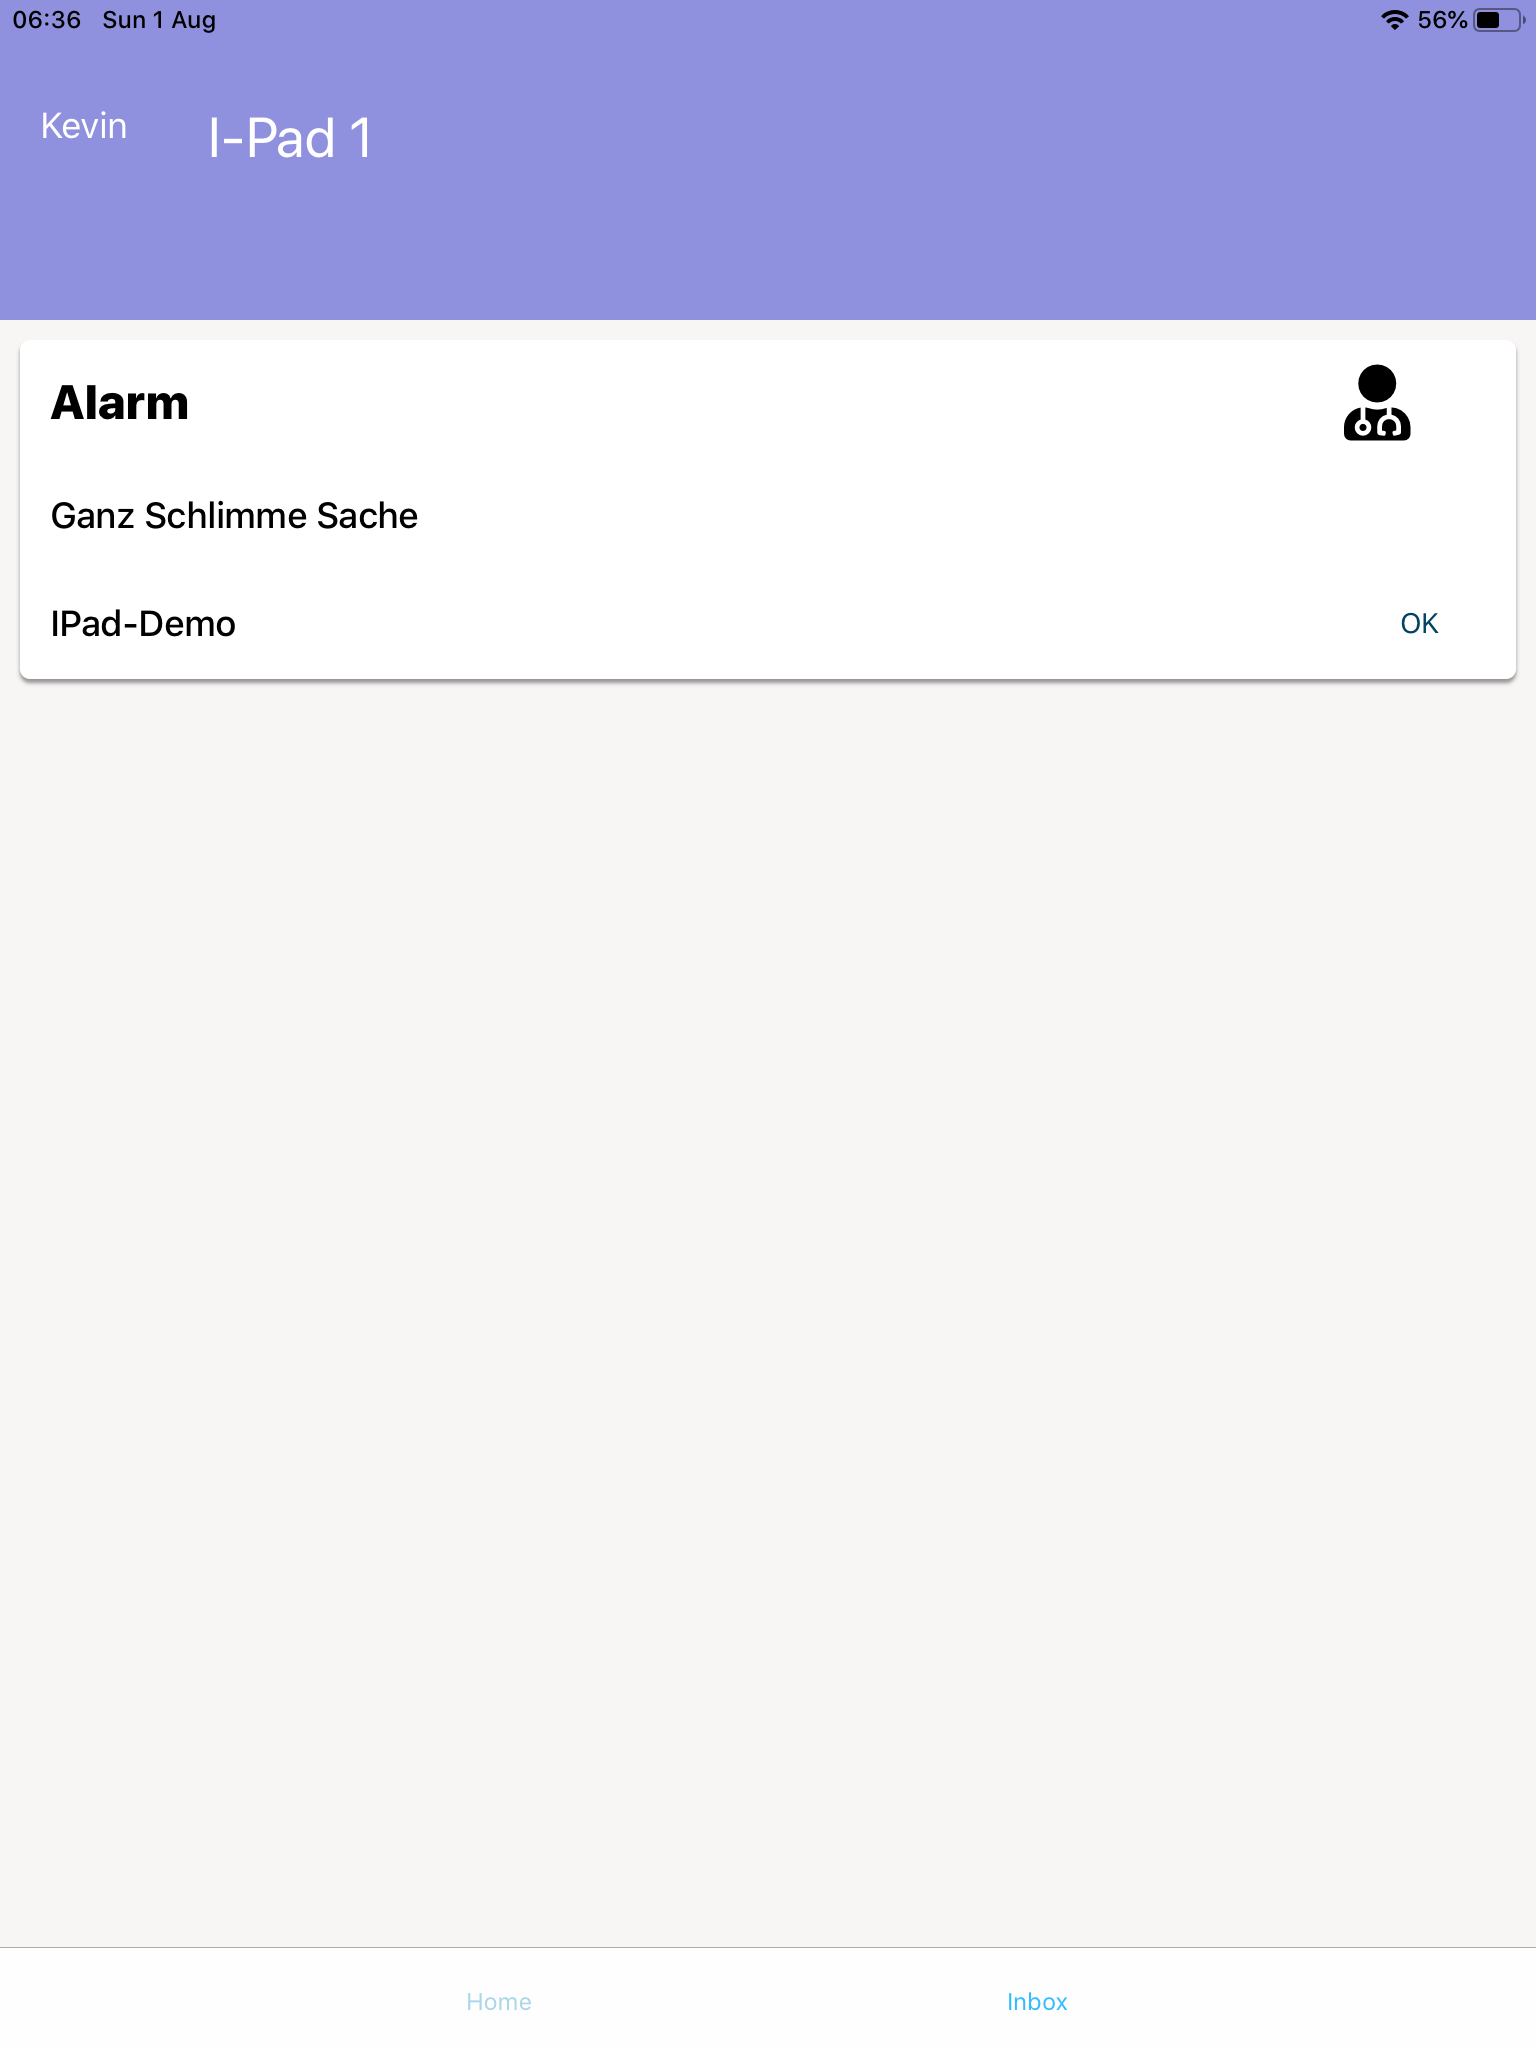
\includegraphics[width=\textwidth]{graphics/screenshots/mobileclient/screenshots-inbox}
        \caption{Inbox}
    \end{minipage}
    \hfill
    \begin{minipage}[b]{0.4\textwidth}
        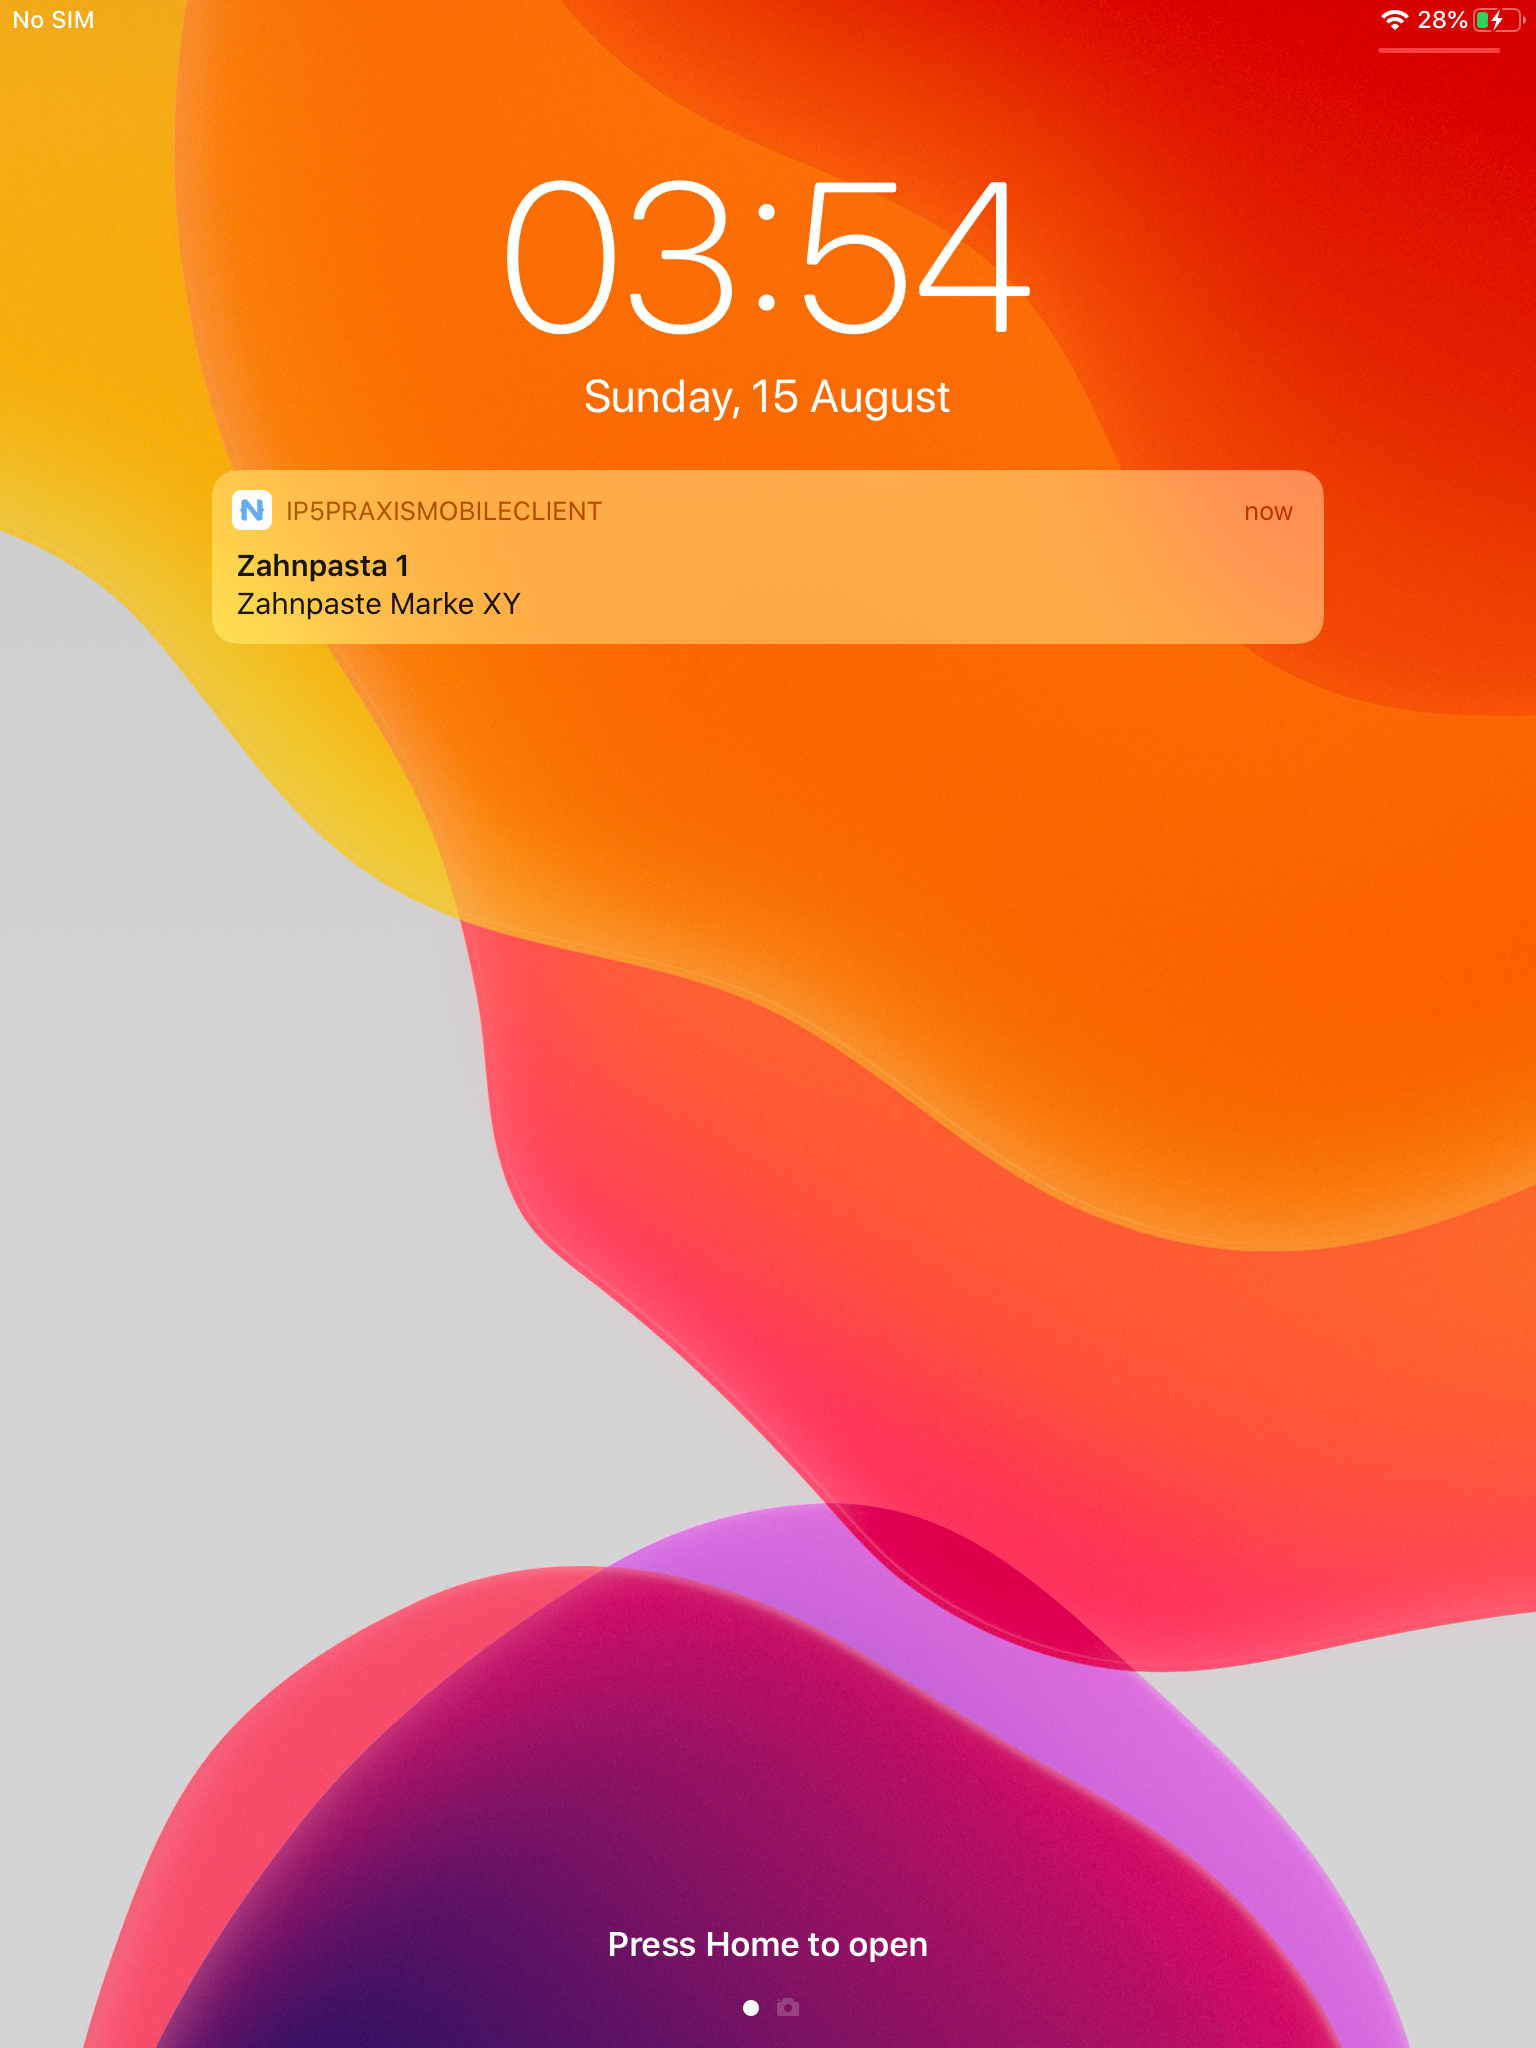
\includegraphics[width=\textwidth]{graphics/screenshots/mobileclient/screenshot-push}
        \caption{Push Benachrichtigung}
    \end{minipage}
    \label{fig:MobileClient-Screens3}
\end{figure}

\clearpage


        
\subsection{Cloud Service}\label{subsec:cloud-service}

\subsubsection{Architektur}

Es gibt deren Domänen 2. Configuration und Notification.

So quasi als ob man 2 Microservices haben kann. Aber wär halt doof das für den stand jetzt schon so zu trennen, deshalb vorerst mal erst ein einzelnes.

\clearpage

\subsubsection{Domänenmodell}


Für die beiden Domänen gibt es natürlich auch so n paar Diagramme. Die gibts jetzt hier:


\subsubsection*{Domäne Configuration}

\begin{figure}[h]
    \centering
    \begin{minipage}[b]{1.0\textwidth}
        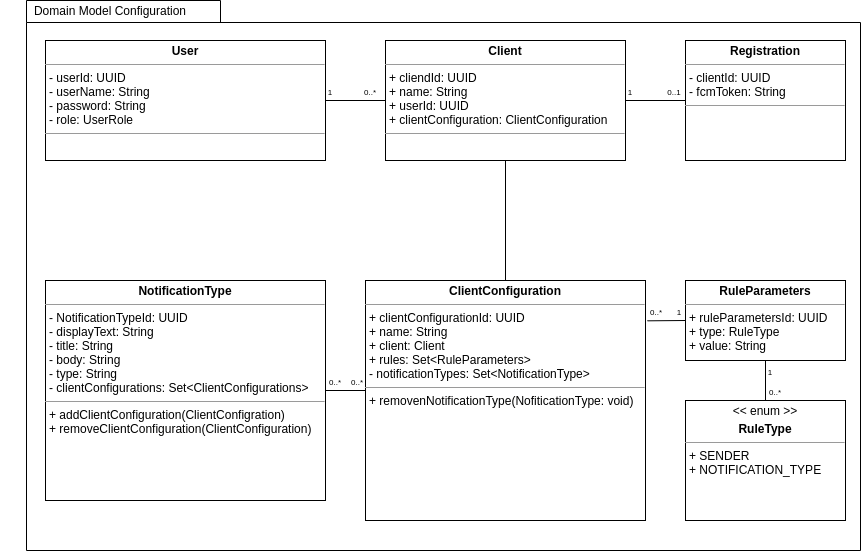
\includegraphics[width=\textwidth]{graphics/Class_Configuration_Domain}
        \caption{Domänenmodell Configuration}
    \end{minipage}
\end{figure}

\clearpage
\subsubsection*{Domäne Notification}

\begin{figure}[h]
    \centering
    \begin{minipage}[b]{1.0\textwidth}
        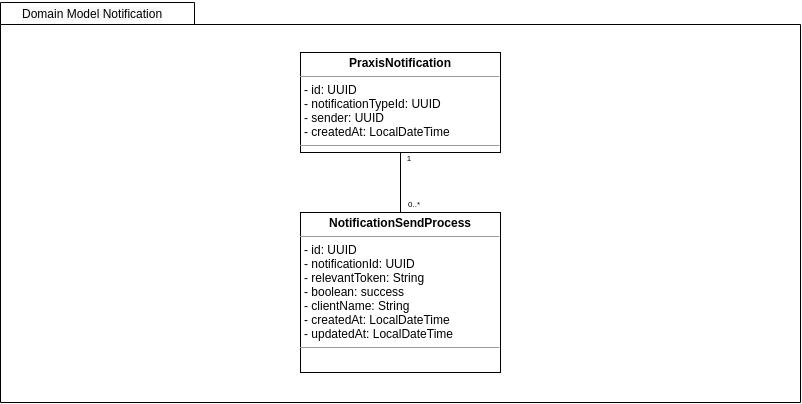
\includegraphics[width=\textwidth]{graphics/Class_Notification_Domain}
        \caption{Domänenmodell Notification}
    \end{minipage}
\end{figure}

\clearpage
\subsubsection*{Rules Engine}

Strategy Pattern mit Spring is noch nice.

\begin{figure}[h]
    \centering
    \begin{minipage}[b]{1.0\textwidth}
        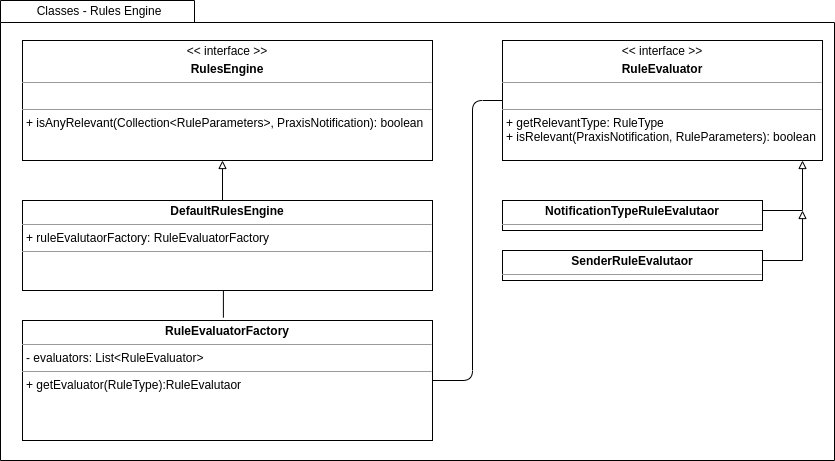
\includegraphics[width=\textwidth]{graphics/Class_Configuration_RulesEngine}
        \caption{Klassendiagramm Rules Engine}
    \end{minipage}
\end{figure}



\clearpage
\subsubsection{API}

S gibt da n paar controller und die brauchen ein paar services.

\clearpage
\subsubsection{Laufzeitmodell}

\clearpage

        \subsubsection{Admin UI}

Das Admin UI bietet Praxisverantwortlichen die Möglichkeit die Konfiguration des Praxisrufsystems zu verwalten.
Da nur Praxisverantworliche das Admin UI verwenden dürfen, ist die Benutzeroberfläche durch ein Login geschützt.
Die entsprechenden Anmeldeinformationen müssen bei Installation des Cloud Services vom Betreiber manuell konfiguriert werden.\footnote{Siehe Anhang D}

\begin{figure}[h]
    \centering
    \begin{minipage}[b]{0.4\textwidth}
        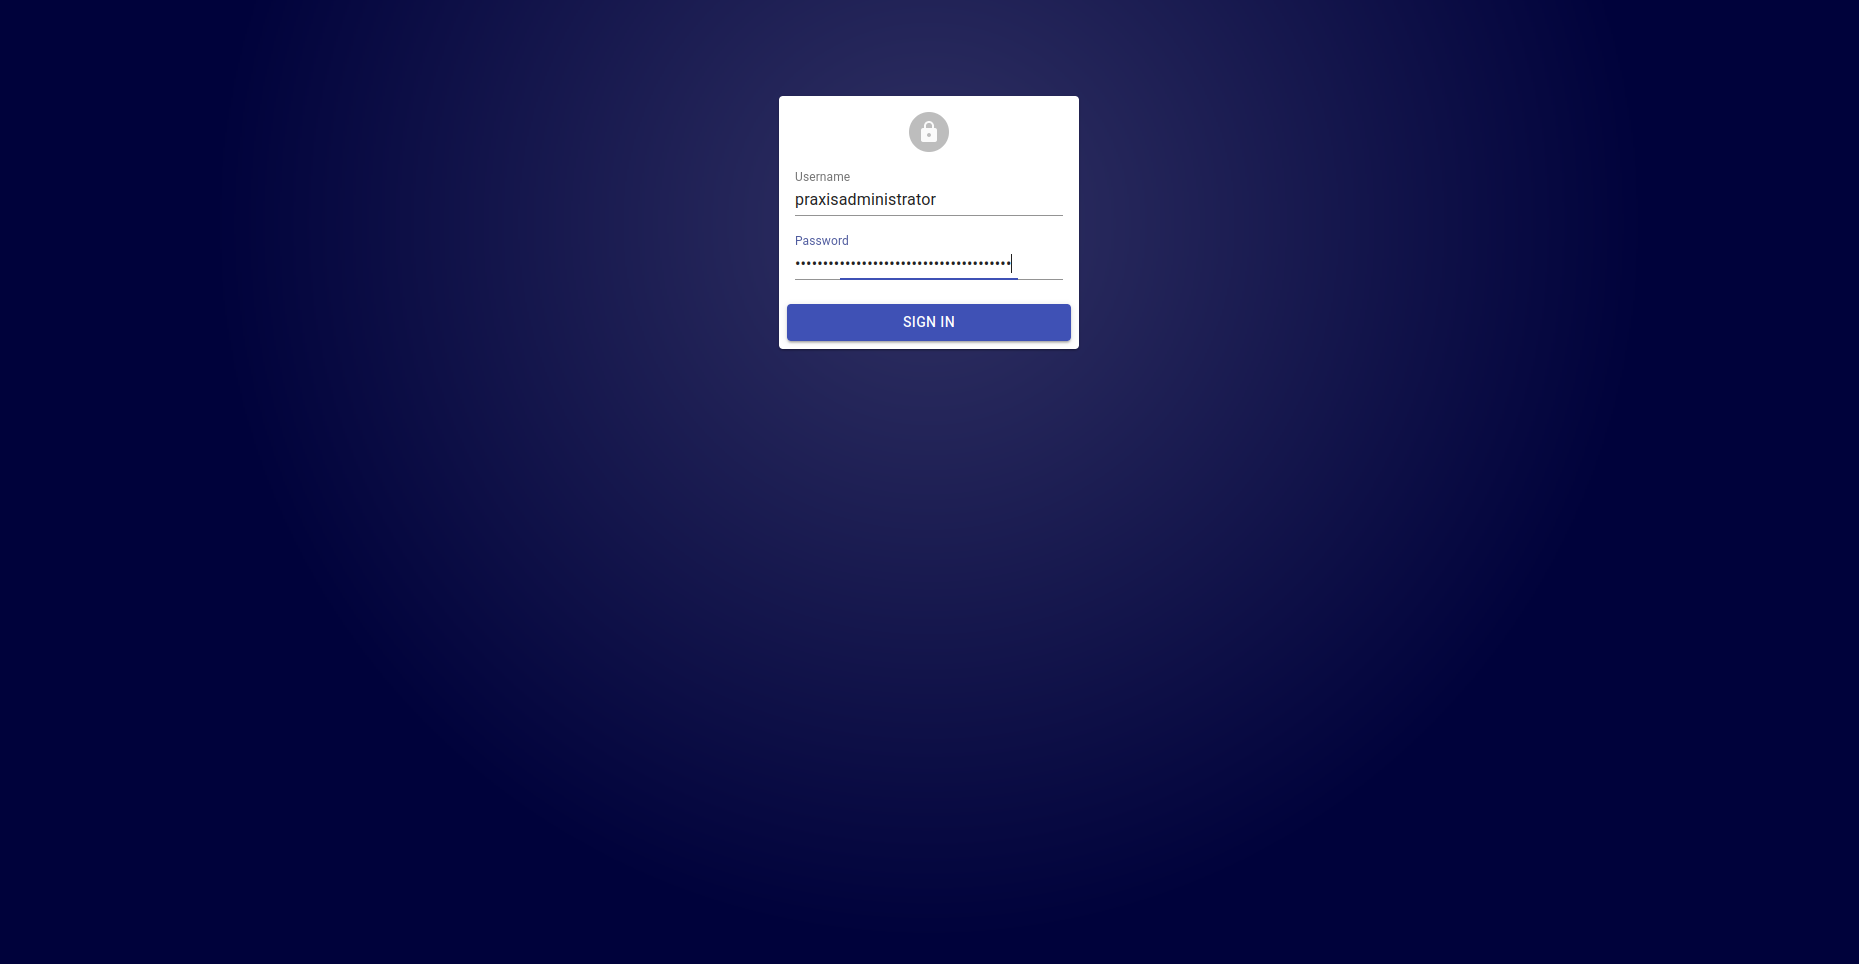
\includegraphics[width=\textwidth]{graphics/screenshots/adminui/login}
        \caption{Login}
    \end{minipage}
    \hfill
    \begin{minipage}[b]{0.4\textwidth}
        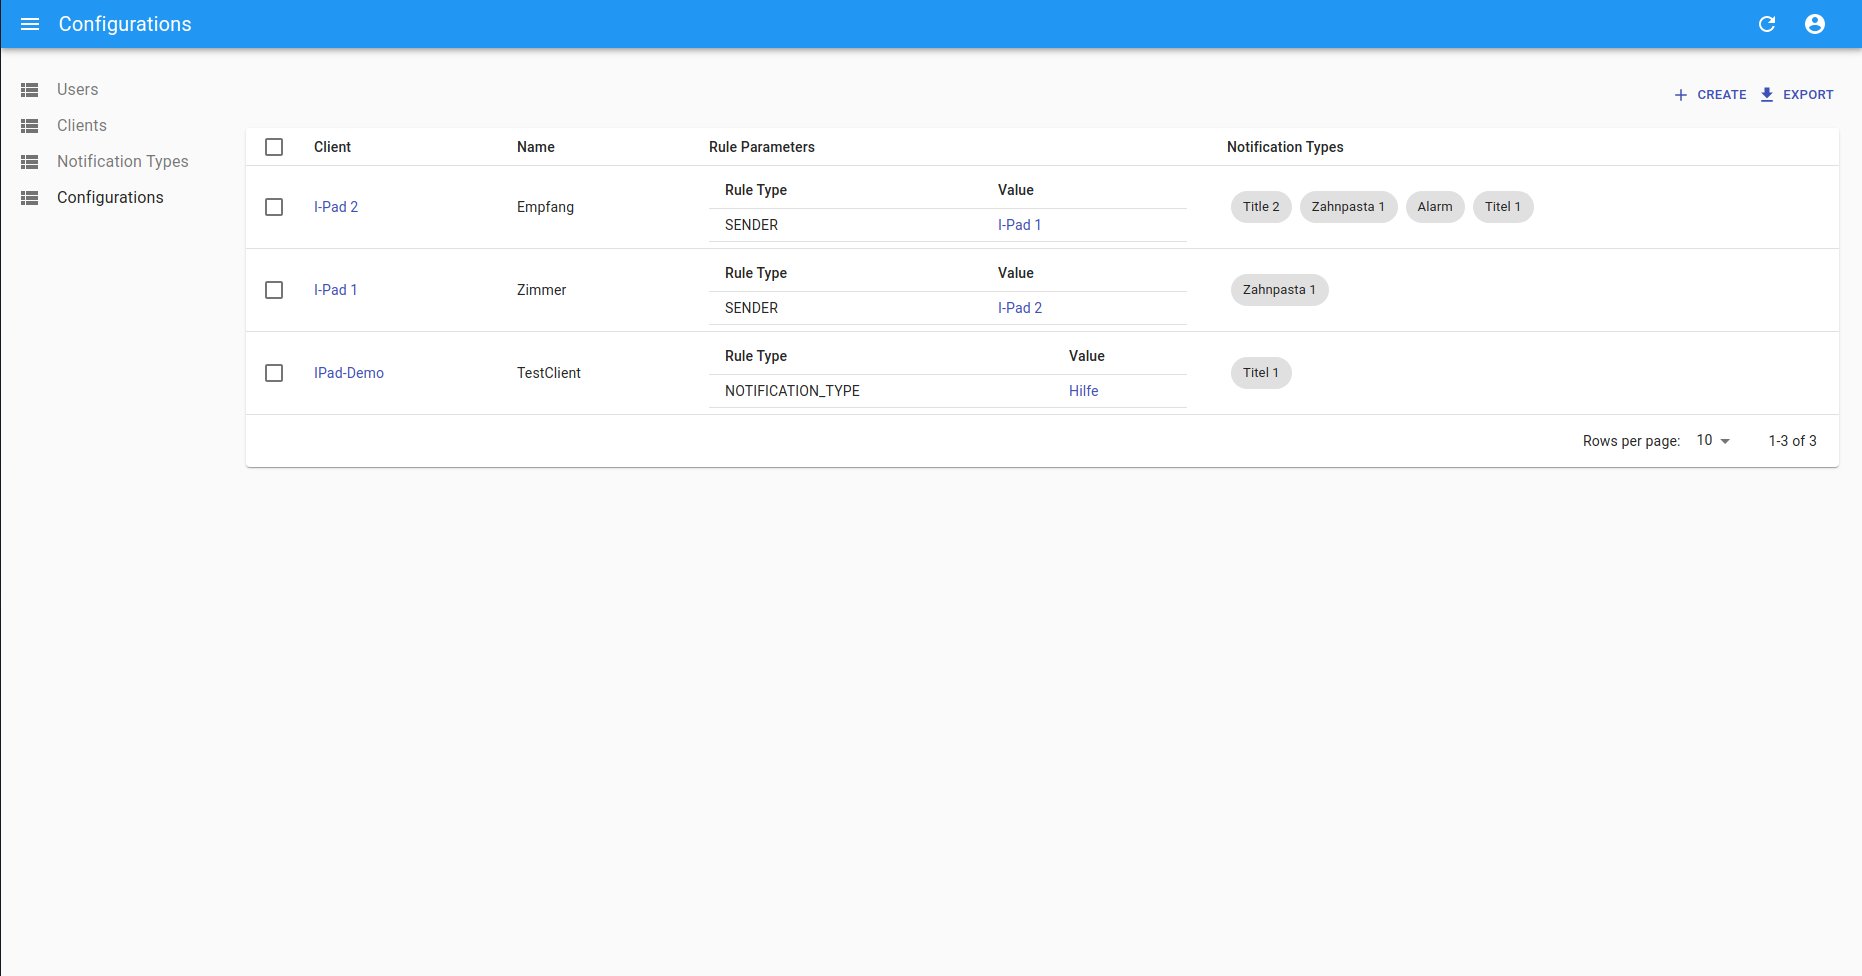
\includegraphics[width=\textwidth]{graphics/screenshots/adminui/configuration-all}
        \caption{Configuration Overview}
    \end{minipage}
    \label{fig:AdminUI-Screens1}
\end{figure}

Das Admin UI beinhaltet vier Bereiche.
Der Bereich Users dient dazu Benutzer zu erstellen, welche sich als Benutzer am Mobile Client anmelden können.
Unter dem Bereich Clients können Geräte verwaltet werden.
Jeder Client ist eindeutig einem Benutzer zugewiesen.
Im Bereich Notification Types können Benachrichtigungen verwaltet werden.
Hier wird konfiguriert, welchen Text der Button für diese Benachrichtigungen im Mobile Client hat und welchen Inhalt die Benachrichtigung hat, wenn sie versendet wird.
Unter dem Bereich Configurations wird die zentrale Konfiguration eines Clients verwaltet.
Jede Konfiguration wird genau einem Client zugewiesen.
Die Konfiguration beinhaltet eine Liste von Notification Types, welche auf dem zugewiesenen Mobile Client als Versenden Button angezeigt werden.
Weiter definiert die Konfiguration eine Liste von Regel Parametern, welche bestimmen, welche Benachrichtigungen dem zugewiesenen Client weitergeleitet werden.

\begin{figure}[h]
    \centering
    \begin{minipage}[b]{0.4\textwidth}
        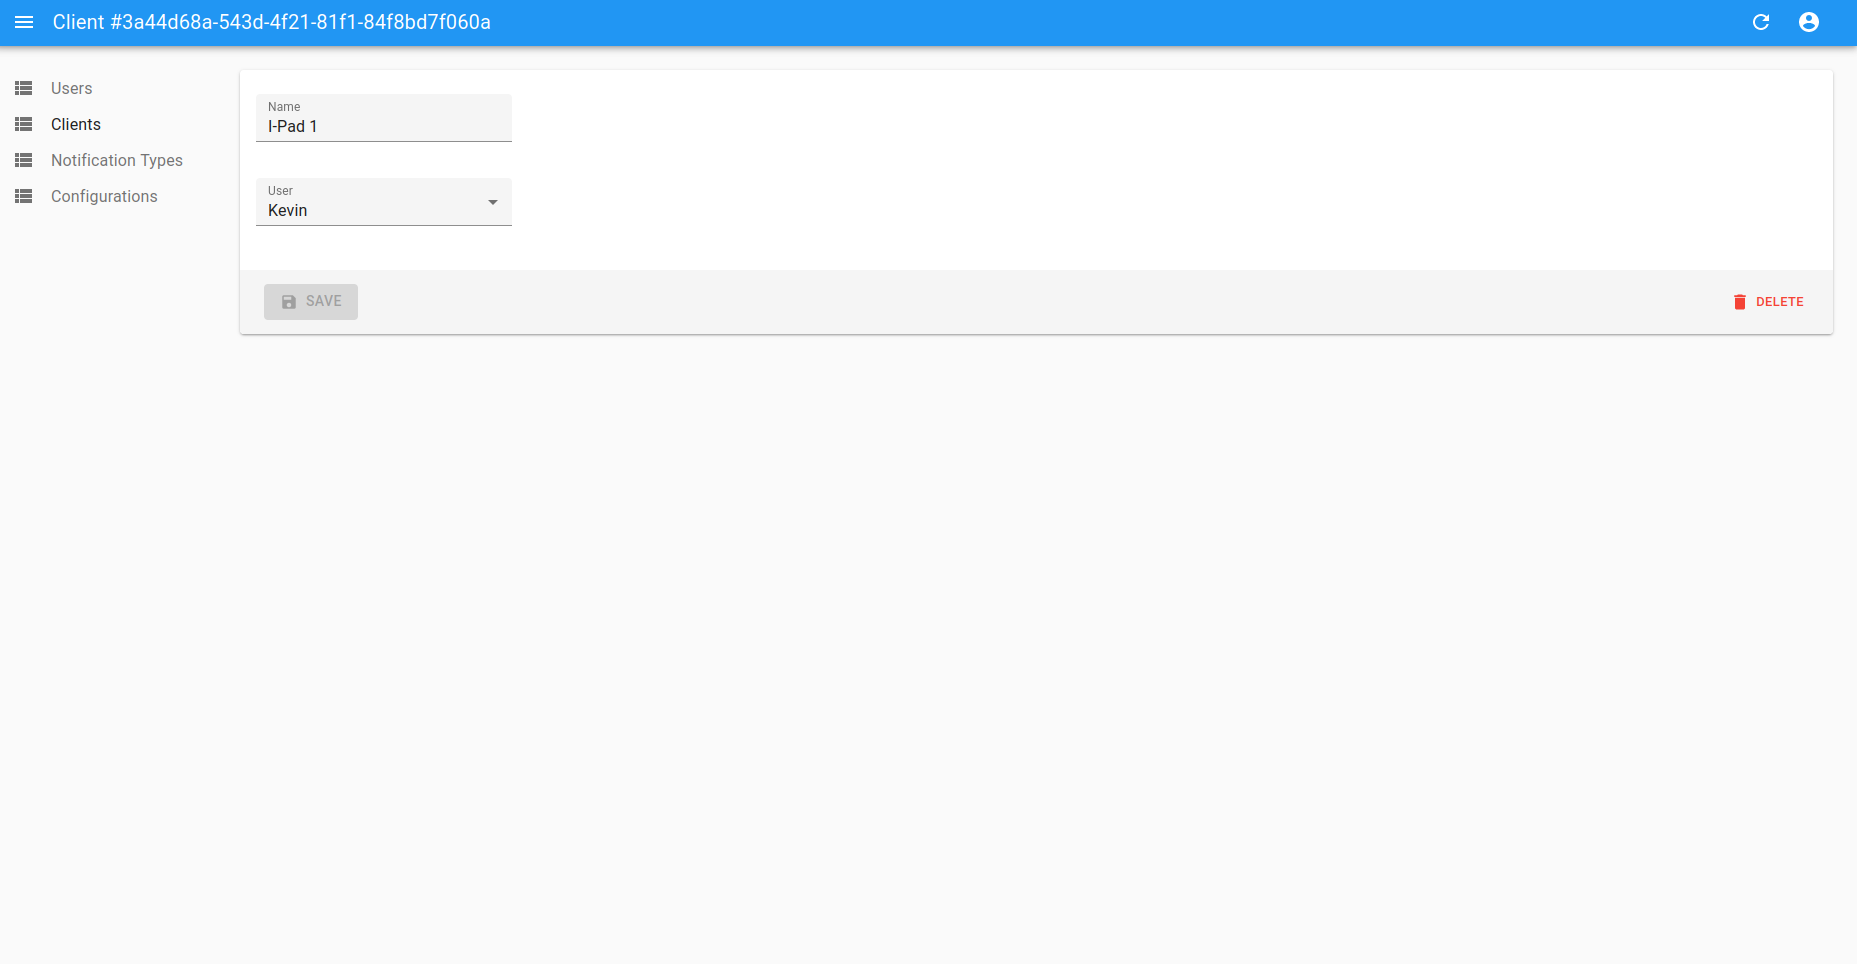
\includegraphics[width=\textwidth]{graphics/screenshots/adminui/configuration}
        \caption{Login}
    \end{minipage}
    \hfill
    \begin{minipage}[b]{0.4\textwidth}
        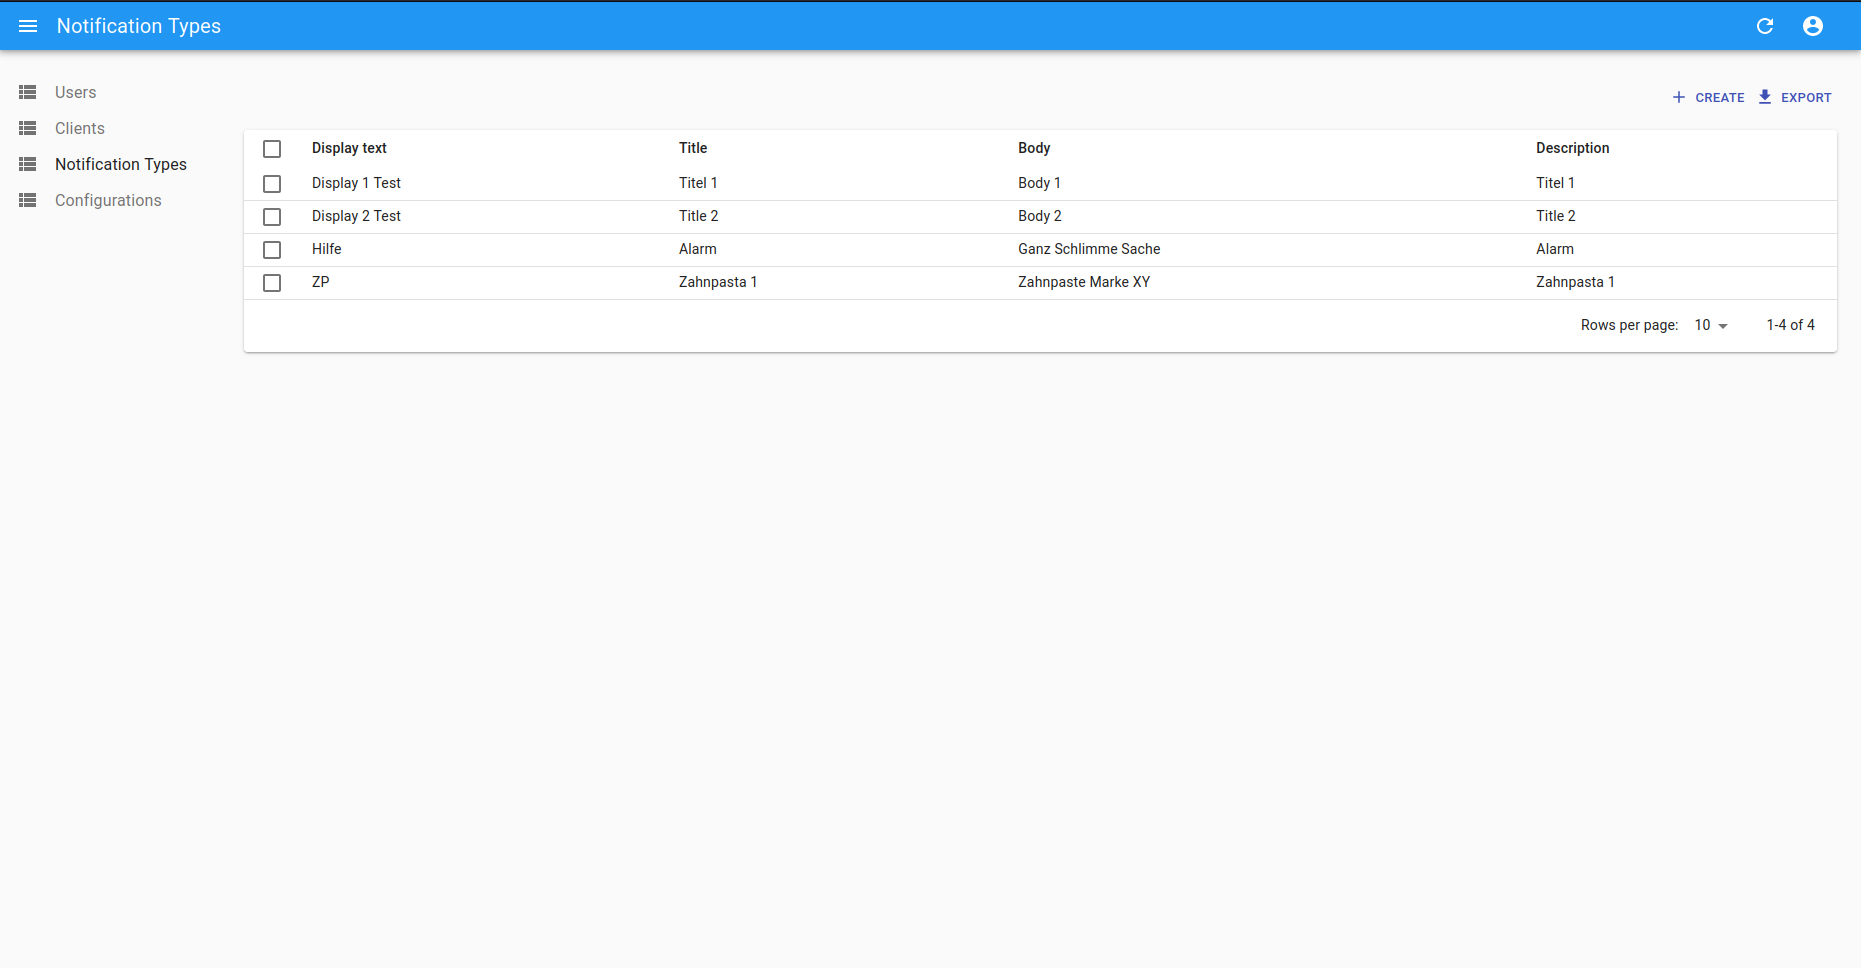
\includegraphics[width=\textwidth]{graphics/screenshots/adminui/notification-type}
        \caption{Configuration Overview}
    \end{minipage}
    \label{fig:AdminUI-Screens2}
\end{figure}

Jeder der Bereiche im Admin UI bietet dem Benutzer die Möglichkeit, den jeweiligen Teil der Konfiguration zu lesen, erstellen, bearbeiten und löschen.
Auf der Startseite jedes Bereiches wird eine Liste mit allen relevanten Einträgen angezeigt.
Mehr Informationen zur Bedienung des Admin UIs befinden sich im Benutzerhandbuch.\footnote{Siehe Anhang C}

\clearpage


    \subsection{Tests}

        \subsubsection*{Benutzertests}

\subsubsection*{Testablauf}

Am 21. Juli 2021 wurden zusammen mit dem Auftraggeber Benutzertests durchgeführt.
Dazu wurde der Mobile Client auf in physisches Ipad installiert.
Zusätzlich wurde eine zweite Mobile Client Instanz auf einem Emulator gestartet.
Der Cloud Service sowie das Admin UI wurden mit Amazon Webservices deployt.
Ein Firebase Messaging Service wurde angebunden.

Für die Benutzertests wurde folgender Ablauf durchgespielt:

\begin{enumerate}
    \item Client 1 im Admin UI anlegen und Benutzer 1 zuweisen.
    \item Client 2 im Admin UI anlegen und Benutzer 1 zuweisen.
    \item Einen neuen Notification Type im Admin UI anlegen
    \item Eine Client Configuration für Client 1 erstellen und darauf den erfassten Notification Type setzen.
    \item Eine Client Configuration für Client 2 erstellen und Regel Parameter erfassen, das alle Benachrichtigungen von Client 1 empfangen werden sollen.
    \item Mobile Client auf Ipad starten
    \item Auf Ipad mit Benutzer 1 anmelden.
    \item Auf Ipad Client 2 auswählen.
    \item Mobile Client auf Emulator starten.
    \item Auf Emulator mit Benutzer 1 anmelden.
    \item Auf Emulator Client 1 auswählen.
    \item Auf Emulator Benachrichtigung auslösen.
\end{enumerate}

Der Test wurde zweimal durchgeführt.
Bei der ersten Durchführung war die Mobile Client Applikation auf dem Empfänger Gerät im Vordergrund geöffnet.
Bei der zweiten Durchführung wurde die Mobile Client Applikation auf dem Empfänger Gerät minimiert.
In beiden Fällen wurde erwartet, dass die Benachrichtigung in der Inbox des Empfängers angezeigt wird.
Im zweiten Fall wurde zusätzlich erwartet, dass eine Push-Benachrichtigung angezeigt wird.

Mehr oder frühere Benutzertests konnten aufgrund der pandemischen Situation nicht durchgeführt werden.

\subsubsection*{Feedback vom Benutzer}

Aus den Tests mit dem Benutzer sind folgende zusätzliche Anforderungen hervorgegangen:

\begin{itemize}
    \item Wenn Benachrichtigungen eingehen sollte ein Audiosignal ertönen.
    \item Wenn Benachrichtigungen nicht quittiert werden, soll ein Erinnerungston ertönen.
    \item Wenn Benachrichtigungen quittiert werden, soll der Versender darüber informiert werden.
\end{itemize}

Um diesen Wünschen Gerecht zu werden, wurden die Szenarien S07 und S09 hinzugefügt.\footnote{Siehe Anhang E}
Diese Anforderungen konnten im Rahmen des Projektes umgesetzt werden.
Der dritte Wunsch des Kunden, die Quittierung von Benachrichtigungen an den Sender weitergeleitet wird konnte aus zeitlichen Gründen nicht mehr umgesetzt werden.

\clearpage


        \subsubsection*{Testplan}

Aus den vervollständigten Features und Szenarien wurde der finale Testplan für das umgesetzte System definiert.
Alle Szenarien sind detailliert im Anhang E beschrieben.
Jedes Szenario definiert die erwarteten Vorbedingungen, einen Testschritt und die zu verifizierenden Ergebnisse.
Diese Szenarien dienen als Grundlage für den Testplan, wobei jedes Szenario einen Testfall darstellt.

Folgendes Protokoll zeigt den Stand der letzten Ausführung der Tests am 19.08.2021:

\begin{table}[h]
    \centering
    \begin{tabular}{|l|p{11cm}|c|c|}
        \hline
        \textbf{Szenario} & \textbf{Beschreibung}                                                                                                                                  & \textbf{Resultat} \\
        \hline
        S01         & Benachrichtigung versenden - Empfänger konfiguriert   & +\\
        \hline
        S02         & Benachrichtigung versenden - kein Empfänger & +\\
        \hline
        S03         & Benachrichtigung empfangen.  & +\\
        \hline
        S04         & Fehler beim Versenden anzeigen.  & +\\
        \hline
        S05         & Wiederholen im Fehlerfall bestätigen.  & +\\
        \hline
        S06         & Wiederholen im Fehlerfall abbrechen.  & +\\
        \hline
        S07         & Audiosignal bei Benachrichtigung.   & +\\
        \hline
        S08         & Push Benachrichtigung im Hintergrund.  & +\\
        \hline
        S09         & Erinnerungston für nicht Quittierte Benachrichtigungen.   & +\\
        \hline
        S10         & Start Mobile Client - nicht angemeldet   & +\\
        \hline
        S11         & Start Mobile Client  - angemeldet & +\\
        \hline
        S12         & Anmelden mit korrekten Daten.   & +\\
        \hline
        S13         & Anmeldung mit ungültigen Daten.   & +\\
        \hline
        S14         & Konfiguration Wählen   & +\\
        \hline
        S15         & Abmelden.   & +\\
        \hline
        S16         & Admin UI - Anmeldung mit korrekten Daten   & +\\
        \hline
        S17         & Admin UI - Anmeldung mit ungültigen Daten   & +\\
        \hline
        S18         & Admin UI - Konfiguration Verwalten   & +\\
        \hline
    \end{tabular}\label{tab:testplan}
\end{table}
\clearpage






\subsubsection*{Performancetests}
Macht nicht so viel sinn mit nur einem Ipad.

\clearpage
\subsection{Herausforderungen}
\begin{itemize}
    \item Dokumentation fehlt komplett in der Planung
    \item IOS Recherche viel aufwändiger als erwartet.
    \item Nativescript aufwändiger zu gebrauchen als erwartet.
    \item AWS aufsetzen ist alles andere als trivial
    \item Keine Erfahrung mit Mobile Development
    \item Stärkerer Roter Faden von Anfang an hätte geholfen
    \item Mehr testing, viel Mehr Testing.
    \item Refactoring kostet Zeit, kanns aber wert sein.
\end{itemize}

\begin{itemize}
    \item Die Gegensprechanlage ist komplett Weggefallen.
    \subitem Grundsätzlich Stünde eine Lib. für IOS in NS zur Verfügung. Der Android Teil ist da noch "TODO"
    \item Die Rückfärbung der Buttons auf Grün ist weggefallen da der Handshake so nicht implmentiert wurde.
\end{itemize}


\subsection{Lessons Learned}

\begin{itemize}
    \item Gute Planung macht sich bezahlt. (Roter Faden, Doku mit einplanen, Standortbestimmung)
    \item Gute Konzepte machen sich bezahlt.
    \item Best Practices gibt es aus einem Grund. (Nativ ist besser)
    \item DevOps ist schwer.
\end{itemize}





